

%% AAPT Physics Bowl Exams Questions
%%----------------------------------------


%% This section has 58 problems


%% PhysicsBowl 2016
%%----------------------------------------
\element{aapt}{
\begin{question}{bowl-2016-q01}
    Which one of the following choices represents the smallest amount of time?
    \begin{multicols}{2}
    \begin{choices}
        \wrongchoice{1 day}
        \wrongchoice{1 minute}
      \correctchoice{1 second}
        \wrongchoice{1 week}
        \wrongchoice{1 year}
    \end{choices}
    \end{multicols}
\end{question}
}

\element{aapt}{
\begin{question}{bowl-2016-q02}
    The position vs. time graph of an object moving on a horizontal line is shown.
    \begin{center}
    \begin{tikzpicture}
        \begin{axis}[
            axis y line=left,
            axis x line=middle,
            axis line style={->},
            xlabel={time},
            x unit=\si{\second},
            xtick={0,2,4,6,8,10},
            minor x tick num=1,
            ylabel={position},
            y unit=\si{\meter},
            ytick={-5,0,5},
            minor y tick num=4,
            grid=major,
            xmin=0,xmax=10.2,
            ymin=-5.5,ymax=5.5,
            width=0.95\columnwidth,
            height=0.50\columnwidth,
        ]
        %% NOTE: TODO: draw curve
        \addplot[line width=1pt,mark=\empty] plot coordinates { (0,0) (3,4) (5,4) (9,-4) (10,-4) };
        \end{axis}
    \end{tikzpicture}
    \end{center}
    At what time(s) is the object moving with its greatest speed?
    \begin{choices}
      \correctchoice{At time $t = \SI{3.0}{\second}$ only}
        \wrongchoice{At time $t = \SI{3.5}{\second}$ only}
        \wrongchoice{At times $t = \SI{3.5}{\second}$ and $t = \SI{9.0}{\second}$}
        \wrongchoice{At time $t = \SI{7.0}{\second}$ only}
        \wrongchoice{At time $t = \SI{9.0}{\second}$ only}
    \end{choices}
\end{question}
}

\element{aapt}{
\begin{question}{bowl-2016-q03}
    A car accelerates uniformly from \SI{0}{\hour} to \SI{60}{\hour} in \SI{4.50}{\second}.
    Which one of the following choices best represents the acceleration of the car?
    \begin{multicols}{2}
    \begin{choices}
        \wrongchoice{\SI{13.3}{\meter\per\second\squared}}
        \wrongchoice{\SI{9.8}{\meter\per\second\squared}}
        \wrongchoice{\SI{4.8}{\meter\per\second\squared}}
      \correctchoice{\SI{3.7}{\meter\per\second\squared}}
        \wrongchoice{\SI{0.37}{\meter\per\second\squared}}
    \end{choices}
    \end{multicols}
\end{question}
}

\element{aapt}{
\begin{question}{bowl-2016-q04}
    The following four length measurements are recorded:
        \SI{5.4e-1}{\meter}, \SI{5.4e0}{\meter}, \SI{5.40e1}{\meter}, and \SI{5.400e2}{\meter}.
    Which one of the following choices best represents the sum of these values using the rules of significant digits?
    \begin{multicols}{2}
    \begin{choices}
        \wrongchoice{\SI{6e2}{\meter}}
        \wrongchoice{\SI{6.0e2}{\meter}}
        \wrongchoice{\SI{6.00e2}{\meter}}
      \correctchoice{\SI{5.999e2}{\meter}}
        \wrongchoice{\SI{5.9994e2}{\meter}}
    \end{choices}
    \end{multicols}
\end{question}
}

\element{aapt}{
\begin{question}{bowl-2016-q05}
    In the figure shown, the mass $m = \SI{6.0}{\kilo\gram}$ and the mass $M = \SI{14.0}{\kilo\gram}$ are stationary.
    \begin{center}
    \begin{tikzpicture}
        %% Ceiling
        \node[anchor=south,fill,pattern=north east lines,minimum width=4cm, minimum height=0.05cm] at (0,0) {};
        \draw (-2,0) -- (2,0);
        %% Masses
        \node[draw,fill=white!90!black,rectangle,rounded corners=1ex,minimum size=0.75cm,anchor=north] (A) at (-0.75,-2) {$m$};
        \node[draw,fill=white!90!black,rectangle,rounded corners=1ex,minimum size=1.25cm,anchor=north] (B) at (0.75,-4) {$M$};
        %% Rope
        \draw[thick] (A.north) -- (-0.75,-1.0) arc(180:0:0.75) -- (B.north);
        %% Pulley
        \draw (0,-1) circle (0.75);
        \draw[fill=white!90!black] (-0.3,0) -- (-0.2,-1.1) arc(190:350:0.2) -- (0.3,0) --cycle;
        \draw[fill] (0,-1) circle (1.5pt);
        %% Floor
        \node[anchor=north,fill,pattern=north east lines,minimum width=4cm, minimum height=0.05cm] at (0,-5.25) {};
        \draw (-2,-5.25) -- (2,-5.25);
    \end{tikzpicture}
    \end{center}
    The mass $M$ rests on the floor.
    Which one of the following choices represents the tension in the string connecting the masses?
    \begin{multicols}{3}
    \begin{choices}
        \wrongchoice{\SI{40}{\newton}}
      \correctchoice{\SI{60}{\newton}}
        \wrongchoice{\SI{80}{\newton}}
        \wrongchoice{\SI{140}{\newton}}
        \wrongchoice{\SI{200}{\newton}}
    \end{choices}
    \end{multicols}
\end{question}
}

\element{aapt}{
\begin{question}{bowl-2016-q06}
    An object, thrown straight downward with a speed of \SI{20.0}{\second},
        takes \SI{2.00}{\second} to reach the ground below.
    From what height above the ground was the object thrown?
    Ignore air resistance.
    \begin{multicols}{3}
    \begin{choices}
        \wrongchoice{\SI{20.0}{\meter}}
        \wrongchoice{\SI{40.0}{\meter}}
        \wrongchoice{\SI{50.0}{\meter}}
      \correctchoice{\SI{60.0}{\meter}}
        \wrongchoice{\SI{80.0}{\meter}}
    \end{choices}
    \end{multicols}
\end{question}
}

\element{aapt}{
\begin{question}{bowl-2016-q07}
    Three cylindrical resistors are made of the same material.
    \begin{center}
    \begin{tikzpicture}
        %% NOTE: TODO: draw resistor
    \end{tikzpicture}
    \end{center}
    The length and radius of each resistor is:
    \begin{description}
        \item[Resistor 1:] Length $L$, radius $r$
        \item[Resistor 2:] Length $L⁄2$ , radius $r⁄2$
        \item[Resistor 3:] Length $L⁄4$ , radius $r⁄2$
    \end{description}
    Which one of the following choices correctly ranks the resistance of these resistors ($R_1$, $R_2$, $R_3$)?
    \begin{multicols}{2}
    \begin{choices}
        \wrongchoice{$R_1 = R_2 < R_3$}
        \wrongchoice{$R_2 < R_1 < R_3$}
        \wrongchoice{$R_3 < R_2 < R_1$}
        \wrongchoice{$R_1 < R_2 = R_3$}
      \correctchoice{$R_1 = R_3 < R_2$}
    \end{choices}
    \end{multicols}
\end{question}
}

\element{aapt}{
\begin{question}{bowl-2016-q08}
    In the history of physics, the names Nicolaus Copernicus, Galileo Galilei, James Clerk Maxwell, and Isaac Newton are very recognizable.
    Which one of the following choices correctly orders these names chronologically by the approximate dates of each person’s scientific work (ending with the most recent)?
    \begin{choices}
      \correctchoice{Copernicus $\rightarrow$ Galileo $\rightarrow$ Newton $\rightarrow$ Maxwell}
        \wrongchoice{Copernicus $\rightarrow$ Galileo $\rightarrow$ Maxwell $\rightarrow$ Newton}
        \wrongchoice{Galileo $\rightarrow$ Copernicus $\rightarrow$ Newton $\rightarrow$ Maxwell}
        \wrongchoice{Galileo $\rightarrow$ Newton $\rightarrow$ Copernicus $\rightarrow$ Maxwell}
        \wrongchoice{Newton $\rightarrow$ Copernicus $\rightarrow$ Maxwell $\rightarrow$ Galileo}
    \end{choices}
\end{question}
}

\element{aapt}{
\begin{question}{bowl-2016-q09}
    In the circuit shown, an electric current exists in the metal resistor connected to the battery.
    \begin{center}
    \ctikzset{bipoles/length=1.00cm}
    \begin{circuitikz}
        %% NOTE: TODO: draw resistor
        \draw (0,0) to [R,l={Resistor}] (4,0) to (4,2) to [battery,l=$V$] (2,2) to (0,2) to (0,0);
    \end{circuitikz}
    \end{center}
    Which one of the following choices best describes the direction of electron flow through the resistor and the direction of the electric field through the interior of the resistor?
    \begin{center}
    \begin{tabu}{cX[c]X[c]}
        \toprule
        \makebox[1.5em][c]{\textnumero}
            & Direction of electron from in resistor
            & Direction of electric field in resistor \\
        \bottomrule
    \end{tabu}
    \end{center}
    \begin{choices}
        \wrongchoice{\begin{tabu}{X[c]X[c]} \tikz \draw[thick,->] (0,0) -- (+1,0); & \tikz \draw[thick,->] (0,0) -- (+1,0); \\ \hline \end{tabu}}
      \correctchoice{\begin{tabu}{X[c]X[c]} \tikz \draw[thick,->] (0,0) -- (-1,0); & \tikz \draw[thick,->] (0,0) -- (+1,0); \\ \hline \end{tabu}}
        \wrongchoice{\begin{tabu}{X[c]X[c]} \tikz \draw[thick,->] (0,0) -- (+1,0); & \tikz \draw[thick,->] (0,0) -- (-1,0); \\ \hline \end{tabu}}
        \wrongchoice{\begin{tabu}{X[c]X[c]} \tikz \draw[thick,->] (0,0) -- (-1,0); & \tikz \draw[thick,->] (0,0) -- (-1,0); \\ \hline \end{tabu}}
        \wrongchoice{\begin{tabu}{X[c]X[c]} \tikz \draw[thick,->] (0,0) -- (+1,0); & There is no electric field \\ \hline \end{tabu}}
    \end{choices}
\end{question}
}

\element{aapt}{
\begin{question}{bowl-2016-q10}
    A person wishes to accelerate an object upward uniformly.
    Which one of the following choices must be true of the force, $F$, provided by the person onto the object?
    $W$ represents the magnitude of the gravitational force acting on the object.
    Ignore any effects of the air or of the Earth's rotation.
    \begin{multicols}{3}
    \begin{choices}
        \wrongchoice{$F = W$}
        \wrongchoice{$F \geq W$}
      \correctchoice{$F > W$}
        \wrongchoice{$F \geq 2W$}
        \wrongchoice{$F > 2W$}
    \end{choices}
    \end{multicols}
\end{question}
}

\element{aapt}{
\begin{question}{bowl-2016-q11}
    A \SI{12.0}{\newton} net force directed to the right is exerted on a \SI{3.0}{\kilo\gram} block for \SI{5.0}{\second}.
    The block was initially at rest and slides on a horizontal surface.
    %% begin question
    What is the speed of the block at the end of the \SI{5.0}{\second} interval?
    \begin{multicols}{3}
    \begin{choices}
        \wrongchoice{\SI{12}{\meter\per\second}}
        \wrongchoice{\SI{15}{\meter\per\second}}
      \correctchoice{\SI{20}{\meter\per\second}}
        \wrongchoice{\SI{36}{\meter\per\second}}
        \wrongchoice{\SI{60}{\meter\per\second}}
    \end{choices}
    \end{multicols}
\end{question}
}

\element{aapt}{
\begin{question}{bowl-2016-q12}
    A \SI{12.0}{\newton} net force directed to the right is exerted on a \SI{3.0}{\kilo\gram} block for \SI{5.0}{\second}.
    The block was initially at rest and slides on a horizontal surface.
    %% begin question
    What is the kinetic energy associated with the block after the \SI{5.0}{\second} interval?
    \begin{multicols}{2}
    \begin{choices}
        \wrongchoice{\SI{180}{\joule}}
      \correctchoice{\SI{600}{\joule}}
        \wrongchoice{\SI{800}{\joule}}
        \wrongchoice{\SI{1200}{\joule}}
        \wrongchoice{\SI{1600}{\joule}}
    \end{choices}
    \end{multicols}
\end{question}
}

\element{aapt}{
\begin{question}{bowl-2016-q13}
    For the inclined plane shown,
    \begin{center}
    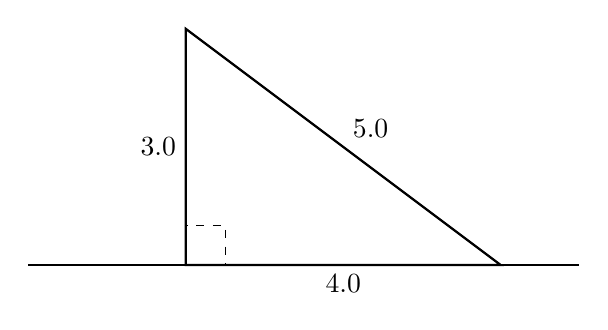
\begin{tikzpicture}
        %% NOTE: TODO: draw pulley
        \draw (-2,0) -- (5,0);
        %% Include
        \draw[thick] (0,0) -- (0,3) -- (4,0) -- cycle;
        \draw[dashed] (0,0) -- (0,0.5) -- (0.5,0.5) -- (0.5,0);
        \draw (0,3) -- (4,0) node[pos=0.5,anchor=south west] {\SI{5.0}{\meter}};
        \draw (0,0) -- (4,0) node[pos=0.5,anchor=north] {\SI{4.0}{\meter}};
        \draw (0,0) -- (0,3) node[pos=0.5,anchor=east] {\SI{3.0}{\meter}};
    \end{tikzpicture}
    \end{center}
        which one of the following choices best represents the value of the incline’s ideal mechanical advantage?
    \begin{multicols}{3}
    \begin{choices}
      \correctchoice{1.67}
        \wrongchoice{1.33}
        \wrongchoice{1.25}
        \wrongchoice{0.80}
        \wrongchoice{0.75}
    \end{choices}
    \end{multicols}
\end{question}
}

\element{aapt}{
\begin{question}{bowl-2016-q14}
    A scientist obtains an answer that has units equivalent to those from computing the square root of the ratio of the Universal Gravitational constant to Coulomb's constant.
    Which one of the following choices has these same units?
    \begin{choices}
        \wrongchoice{energy divided by time}
        \wrongchoice{length divided by time}
        \wrongchoice{mass divided by energy}
        \wrongchoice{electric field strength divided by magnetic field strength}
      \correctchoice{charge divided by mass}
    \end{choices}
\end{question}
}

\element{aapt}{
\begin{question}{bowl-2016-q15}
    A radio station broadcasts its signal at a frequency of \SI{100.0}{\mega\hertz}.
    What is the wavelength of the station's signal?
    \begin{multicols}{3}
    \begin{choices}
        \wrongchoice{\SI{3.00}{\kilo\meter}}
      \correctchoice{\SI{3.00}{\meter}}
        \wrongchoice{\SI{3.00}{\milli\meter}}
        \wrongchoice{\SI{0.33}{\meter}}
        \wrongchoice{\SI{0.33}{\kilo\meter}}
    \end{choices}
    \end{multicols}
\end{question}
}

\element{aapt}{
\begin{question}{bowl-2016-q16}
    A uniform stick is fixed to rotate about an axis through its center.
    The stick starts from rest and rotates through an angle of \ang{90} in a time of \SI{1.0}{\second}.
    If the angular acceleration of the stick is constant,
        what is the angular speed of the stick about its rotation axis after one full revolution?
    \begin{multicols}{3}
    \begin{choices}
        \wrongchoice{\SI[parse-numbers=false]{4\pi}{\radian\per\second}}
        \wrongchoice{\SI[parse-numbers=false]{4\sqrt{2}\pi}{\radian\per\second}}
      \correctchoice{\SI[parse-numbers=false]{2\pi}{\radian\per\second}}
        \wrongchoice{\SI[parse-numbers=false]{\sqrt{2}\pi}{\radian\per\second}}
        \wrongchoice{\SI[parse-numbers=false]{\pi}{\radian\per\second}}
    \end{choices}
    \end{multicols}
\end{question}
}

\element{aapt}{
\begin{question}{bowl-2016-q17}
    ``All planets in the solar system follow elliptical orbits with the Sun located at one focus of the ellipse.''
    This statement is best summarized by which one of the following choices?
    \begin{choices}
      \correctchoice{Kepler's First Law}
        \wrongchoice{Kepler's Second Law}
        \wrongchoice{Newton's Universal Law of Gravitation}
        \wrongchoice{Einstein's Law of Gravity}
        \wrongchoice{Schwarzchild's Law of Orbits}
    \end{choices}
\end{question}
}

\element{aapt}{
\begin{question}{bowl-2016-q18}
    For any motion in two dimensions, which one of the following choices identifies quantities that must have the same direction?
    \begin{choices}
      \correctchoice{average velocity and displacement}
        \wrongchoice{average acceleration and average velocity}
        \wrongchoice{average acceleration and displacement}
        \wrongchoice{final velocity and average acceleration}
        \wrongchoice{final velocity and displacement}
    \end{choices}
\end{question}
}

\element{aapt}{
\begin{question}{bowl-2016-q19}
    An ideal gas in a sealed container with \num{1.20e24} particles has a pressure of \SI{1.0}{\atm} at a temperature of \SI{27.0}{\degreeCelsius}.
    Which one of the following choices best represents the volume of the container?
    \begin{multicols}{2}
    \begin{choices}
        \wrongchoice{\SI{450}{\meter\cubed}}
        \wrongchoice{\SI{4.5}{\meter\cubed}}
        \wrongchoice{\SI{0.49}{\meter\cubed}}
      \correctchoice{\SI{0.049}{\meter\cubed}}
        \wrongchoice{\SI{0.00049}{\meter\cubed}}
    \end{choices}
    \end{multicols}
\end{question}
}

\element{aapt}{
\begin{question}{bowl-2016-q20}
    A uniform \SI{10.0}{\meter} long plank is pivoted about its center of gravity.
    A mass $M_1$ then is placed at the left edge of the plank and a second mass $M_2$ is placed \SI{1.0}{\meter} from the right end.
    This system is in static equilibrium (shown).
    \begin{center}
    \begin{tikzpicture}
        %% NOTE: TODO: draw pulley
    \end{tikzpicture}
    \end{center}
    If each mass now is moved \SI{2.0}{\meter} closer to the center of the plank,
        which one of the following choices best describes the subsequent motion of the plank?
    \begin{choices}
        \wrongchoice{The plank remains in static equilibrium.}
        \wrongchoice{The plank rotates at constant angular speed until the right side reaches the ground.}
        \wrongchoice{The plank rotates at constant angular speed until the left side reaches the ground.}
        \wrongchoice{The plank angularly accelerates until the right side reaches the ground.}
      \correctchoice{The plank angularly accelerates until the left side reaches the ground.}
    \end{choices}
\end{question}
}

\element{aapt}{
\begin{question}{bowl-2016-q21}
    At \SI{1.94}{\second} after launch, a projectile in free fall achieved its minimum speed during flight.
    If that minimum speed was \SI{15.0}{\meter\per\second},
        what was the projectile's initial angle of launch from the horizontal?
    \begin{multicols}{3}
    \begin{choices}
        \wrongchoice{\ang{82.6}}
      \correctchoice{\ang{52.3}}
        \wrongchoice{\ang{50.6}}
        \wrongchoice{\ang{39.4}}
        \wrongchoice{\ang{37.7}}
    \end{choices}
    \end{multicols}
\end{question}
}

\element{aapt}{
\begin{question}{bowl-2016-q22}
    For the following nuclear reaction,
    \begin{equation}
        \ce{^{40}_{19}K + e^- -> $X$ + ^{0}_{0} \nu_e }
    \end{equation}
        which one of the following choices correctly identifies the quantity labeled $X$?
    \begin{multicols}{3}
    \begin{choices}
        \wrongchoice{\ce{^{40}_{19}K}}
        \wrongchoice{\ce{^{40}_{18}K}}
        \wrongchoice{\ce{^{39}_{18}Ar}}
        \wrongchoice{\ce{^{39}_{19}K}}
      \correctchoice{\ce{^{40}_{18}Ar}}
    \end{choices}
    \end{multicols}
\end{question}
}

\element{aapt}{
\begin{question}{bowl-2016-q23}
    At a party, two spherical balloons are expanded to have the same radius.
    Balloon \#1 is filled with helium gas while balloon \#2 is filled with xenon gas.
    Which one of the following statements about the buoyant forces on the balloons is correct?
    \begin{choices}
        \wrongchoice{The buoyant force is greater for the helium balloon.}
        \wrongchoice{The buoyant force is greater for the xenon balloon.}
      \correctchoice{The buoyant force is the same for each balloon.}
        \wrongchoice{The balloon experiencing the greater buoyant force cannot be determined without knowing the radius .}
        \wrongchoice{The balloon experiencing the greater buoyant force cannot be determined without knowing the atmospheric pressure at the time.}
    \end{choices}
\end{question}
}

\element{aapt}{
\begin{question}{bowl-2016-q24}
    A proton moves with constant non-zero velocity in a region of space that has a uniform magnetic field directed into the plane of the page.
    The proton moves directly up the plane of the page.
    What is the direction of the electric field in this region of space?
    Ignore gravity.
    \begin{choices}
        \wrongchoice{To the left}
      \correctchoice{To the right}
        \wrongchoice{Down the plane of the page}
        \wrongchoice{Up the plane of the page}
        \wrongchoice{There is no electric field necessary}
    \end{choices}
\end{question}
}

\element{aapt}{
\begin{question}{bowl-2016-q25}
    The plates of a large parallel-plate capacitor are separated by a distance of \SI{0.05}{\meter}.
    The potential difference between the plates is \SI{24.0}{\volt}.
    A charge released from rest between the plates experiences an electric force of \SI{1.00}{\newton}.
    What is the magnitude of the charge released between the plates?
    \begin{multicols}{3}
    \begin{choices}
      \correctchoice{\SI{2.08}{\milli\coulomb}}
        \wrongchoice{\SI{4.17}{\milli\coulomb}}
        \wrongchoice{\SI{8.33}{\milli\coulomb}}
        \wrongchoice{\SI{16.6}{\milli\coulomb}}
        \wrongchoice{\SI{33.3}{\milli\coulomb}}
    \end{choices}
    \end{multicols}
\end{question}
}

\element{aapt}{
\begin{question}{bowl-2016-q26}
    A \SI{10.0}{\kilo\gram} mass moves to the right at \SI{8.00}{\second}.
    A \SI{5.0}{\kilo\gram} mass moves to the left at \SI{7.00}{\second}.
    With what speed does the center of mass of this two-mass system move?
    \begin{multicols}{3}
    \begin{choices}
        \wrongchoice{\SI{7.67}{\meter\per\second}}
        \wrongchoice{\SI{7.50}{\meter\per\second}}
      \correctchoice{\SI{3.00}{\meter\per\second}}
        \wrongchoice{\SI{2.00}{\meter\per\second}}
        \wrongchoice{\SI{0.50}{\meter\per\second}}
    \end{choices}
    \end{multicols}
\end{question}
}

\element{aapt}{
\begin{question}{bowl-2016-q27}
    A tuning fork of frequency $f$ is placed over a long tube closed at one end producing the third lowest frequency standing wave for the tube.
    What frequency tuning fork would be needed to produce the fourth lowest frequency standing wave?
    \begin{multicols}{3}
    \begin{choices}
        \wrongchoice{$\dfrac{4f}{3}$}
        \wrongchoice{$\dfrac{5f}{3}$}
        \wrongchoice{$\dfrac{6f}{5}$}
      \correctchoice{$\dfrac{7f}{5}$}
        \wrongchoice{$\dfrac{5f}{4}$}
    \end{choices}
    \end{multicols}
\end{question}
}

\element{aapt}{
\begin{question}{bowl-2016-q28}
    Recent excitement in the physics community came from the February, 2016 announcement from LIGO that:
    \begin{choices}
        \wrongchoice{alien life had been discovered on a distant planet.}
        \wrongchoice{dark matter had been discovered.}
        \wrongchoice{there was proof of dark energy’s existence.}
      \correctchoice{gravitational waves had been detected.}
        \wrongchoice{objects had been observed to travel faster than the speed of light.}
    \end{choices}
\end{question}
}

\element{aapt}{
\begin{question}{bowl-2016-q29}
    A ray of light is incident onto a thin glass lens as shown.
    \begin{center}
    \begin{tikzpicture}
        %% NOTE: TODO: draw ray diagram
    \end{tikzpicture}
    \end{center}
    Which one of the following arrows best indicates the path of the refracted ray?
    \begin{multicols}{5}
    \begin{choices}[o]
        \wrongchoice{$A$}
        \wrongchoice{$B$}
        \wrongchoice{$C$}
        \wrongchoice{$D$}
      \correctchoice{$E$}
    \end{choices}
    \end{multicols}
\end{question}
}

\element{aapt}{
\begin{question}{bowl-2016-q30}
    A scientist wishes to compute the amount of energy necessary to melt a known mass of a solid sample.
    Which quantity associated with the sample would the scientist be most interested in knowing?
    \begin{choices}
      \correctchoice{Latent heat of fusion}
        \wrongchoice{Specific heat}
        \wrongchoice{Coefficient of thermal expansion}
        \wrongchoice{Latent heat of vaporization}
        \wrongchoice{Thermal conductivity}
    \end{choices}
\end{question}
}

\element{aapt}{
\begin{question}{bowl-2016-q31}
    The circuit shown has 4 identical light bulbs connected to an ideal battery.
    \begin{center}
    \begin{circuitikz}
        %% NOTE: TODO: draw circuit
    \end{circuitikz}
    \end{center}
    If bulb \#2 were removed leaving an open circuit there,
        what happens to the voltage across both bulb \#1 and from $Q$ to $X$?
    \begin{center}
    \begin{tabu}{cX[c]X[c]}
        \toprule
        \makebox[1.5em][c]{\textnumero}
            & Voltage across bulb \#1
            & Voltage from $Q$ to $X$ \\
        \bottomrule
    \end{tabu}
    \end{center}
    \begin{choices}
        \wrongchoice{\begin{tabu}{X[c]X[c]} Remains the same & Decreases \\ \end{tabu}}
        \wrongchoice{\begin{tabu}{X[c]X[c]} Decreases        & Remains the same \\ \end{tabu}}
        \wrongchoice{\begin{tabu}{X[c]X[c]} Increases        & Decreases \\ \end{tabu}}
        \wrongchoice{\begin{tabu}{X[c]X[c]} Increases        & Increases \\ \end{tabu}}
      \correctchoice{\begin{tabu}{X[c]X[c]} Decreases        & Increases \\ \end{tabu}}
    \end{choices}
\end{question}
}

\element{aapt}{
\begin{question}{bowl-2016-q32}
    A mass connected to a string forms a simple pendulum.
    The mass is released from rest and undergoes simple harmonic motion.
    Which one of the following choices correctly ranks the magnitude of the tension in the string ($T$),
        the gravitational force on the mass ($W$),
        and the net force acting on the mass ($F$) when the mass swings through its lowest point?
    \begin{multicols}{2}
    \begin{choices}
        \wrongchoice{$F < W = T$}
        \wrongchoice{$W < T < F$}
        \wrongchoice{$W < F = T$}
      \correctchoice{$F < W < T$}
        \wrongchoice{More information is required to answer the question.}
    \end{choices}
    \end{multicols}
\end{question}
}

\element{aapt}{
\begin{question}{bowl-2016-q33}
    Given the configuration of three charges, $+Q$, $+Q$, and $-2Q$,
    \begin{center}
    \begin{tikzpicture}
        %% NOTE: TODO: draw charge diagram
    \end{tikzpicture}
    \end{center}
        which one of the following choices best represents the direction of the electric field at the point $P$ and the sign of the electric potential at $P$ from these charges?
    \begin{center}
    \begin{tabu}{cX[c]X[c]}
        \toprule
        \makebox[1.5em][c]{\textnumero}
            & Field Direction at $P$ & Sign of Electric Potential at $P$ \\
        \bottomrule
    \end{tabu}
    \end{center}
    \begin{choices}
        %% NOTE: TODO: Improve alignment
        \wrongchoice{\begin{tabu}{X[c]X[c]} \tikz \draw[thick,-latex] (0,0) -- ++ (+0.714,-0.714); & Positive \\ \hline \end{tabu}}
      \correctchoice{\begin{tabu}{X[c]X[c]} \tikz \draw[thick,-latex] (0,0) -- ++ (-0.714,+0.714); & Positive \\ \hline \end{tabu}}
        \wrongchoice{\begin{tabu}{X[c]X[c]} \tikz \draw[thick,-latex] (0,0) -- ++ (+0.714,-0.714); & Negative \\ \hline \end{tabu}}
        \wrongchoice{\begin{tabu}{X[c]X[c]} \tikz \draw[thick,-latex] (0,0) -- ++ (-0.714,+0.714); & Negative \\ \hline \end{tabu}}
        \wrongchoice{\begin{tabu}{X[c]X[c]} Zero & Zero \\ \hline \end{tabu}}
    \end{choices}
\end{question}
}

\element{aapt}{
\begin{question}{bowl-2016-q34}
    The graph shows the magnitude of the linear momentum of two solid objects colliding on the $x$-axis.
    \begin{center}
    \begin{tikzpicture}
        \begin{axis}[
            axis y line=left,
            axis x line=middle,
            axis line style={->},
            xlabel={time},
            x unit=\si{\second},
            xtick={0,2,4,6,8,10},
            minor x tick num=1,
            ylabel={position},
            y unit=\si{\meter},
            ytick={-5,0,5},
            minor y tick num=4,
            grid=major,
            xmin=0,xmax=10.2,
            ymin=-5.5,ymax=5.5,
            width=0.95\columnwidth,
            height=0.50\columnwidth,
        ]
        %% NOTE: TODO: draw curve
        \addplot[line width=1pt,mark=\empty] plot coordinates { (0,0) (3,4) (5,4) (9,-4) (10,-4) };
        \end{axis}
    \end{tikzpicture}
    \end{center}
    Which one of the following statements must be true based on the information provided?
    \begin{choices}
        \wrongchoice{The objects remain stuck together after the collision.}
        \wrongchoice{Object 2 experiences the greater force from the collision.}
      \correctchoice{Object 2 cannot have more mass than object 1.}
        \wrongchoice{The kinetic energy loss was maximized with no external forces present in the two-object system.}
        \wrongchoice{The kinetic energy of the two-object system is the same both before and after the collision.}
    \end{choices}
\end{question}
}

\element{aapt}{
\begin{question}{bowl-2016-q35}
    Which one of the following choices best describes what it means for an object to be iridescent?
    \begin{choices}
      \correctchoice{The color of the object appears to change with a change in the angle of view.}
        \wrongchoice{The object appears to have two images formed from it because of differences in index of refraction.}
        \wrongchoice{The color of the object appears to be different based on its temperature.}
        \wrongchoice{The object remains illuminated after turning off all surrounding light sources.}
        \wrongchoice{The object is alive and producing light biochemically.}
    \end{choices}
\end{question}
}

\element{aapt}{
\begin{question}{bowl-2016-q36}
    On a straight road, a self-driving car races with a robot.
    The robot accelerates at \SI{8.50}{\meter\per\second\squared} until reaching its maximum constant speed of \SI{15.0}{\meter\per\second}.
    The car accelerates at \SI{5.60}{\meter\per\second\squared} until reaching its maximum constant speed of \SI{25.0}{\meter\per\second}.
    The car and robot start from rest from the same location.
    What is the maximum distance that the robot leads the car during the race?
    \begin{multicols}{3}
    \begin{choices}
        \wrongchoice{\SI{3.3}{\meter}}
      \correctchoice{\SI{6.9}{\meter}}
        \wrongchoice{\SI{10.2}{\meter}}
        \wrongchoice{\SI{13.2}{\meter}}
        \wrongchoice{\SI{17.3}{\meter}}
    \end{choices}
    \end{multicols}
\end{question}
}

\newcommand{\BowlTwentySixteenQThirtySeven}{
    \begin{tikzpicture}
        %% NOTE: TODO: draw charge diagram
    \end{tikzpicture}
}

\element{aapt}{
\begin{question}{bowl-2016-q37}
    %% Questions 37 – 38 deal with the following information:
    A string is connected to a mechanical oscillator on one end and to a cube-shaped mass, $M=\SI{8.0}{\kilo\gram}$, at the other end as shown.
    %% NOTE: change wording: left to below or somehting
    The oscillator vibrates the string with a frequency of $f$ producing the standing wave in the figure on the left.
    When the mass is submerged completely in water,
        the string vibrates in the standing wave pattern shown on the right.
    %% start question
    What is the value of the ratio for the tension when the mass is submerged in water to the tension when the mass is hanging in air?
    \begin{multicols}{3}
    \begin{choices}
        \wrongchoice{$4$}
        \wrongchoice{$2$}
        \wrongchoice{$\dfrac{1}{\sqrt{2}}$}
        \wrongchoice{$\dfrac{1}{2}$}
      \correctchoice{$\dfrac{1}{4}$}
    \end{choices}
    \end{multicols}
\end{question}
}

\element{aapt}{
\begin{question}{bowl-2016-q38}
    %% Questions 37 – 38 deal with the following information:
    A string is connected to a mechanical oscillator on one end and to a cube-shaped mass, $M=\SI{8.0}{\kilo\gram}$, at the other end as shown.
    %% NOTE: change wording: left to below or somehting
    The oscillator vibrates the string with a frequency of $f$ producing the standing wave in the figure on the left.
    When the mass is submerged completely in water,
        the string vibrates in the standing wave pattern shown on the right.
    %% start question
    What is the length of one side of the cube of mass $M$?
    \begin{multicols}{3}
    \begin{choices}
        \wrongchoice{\SI{0.006}{\meter}}
        \wrongchoice{\SI{0.091}{\meter}}
        \wrongchoice{\SI{0.126}{\meter}}
      \correctchoice{\SI{0.182}{\meter}}
        \wrongchoice{\SI{0.200}{\meter}}
    \end{choices}
    \end{multicols}
\end{question}
}

\element{aapt}{
\begin{question}{bowl-2016-q39}
    %% Questions 39 – 40 deal with the following information:
    An object moves in a circle, starting at the top, with initial speed \SI{17.0}{\second} .
    The object's speed increases uniformly until it has moved counterclockwise through an angle of \ang{55}.
    The average acceleration for this motion is \SI{9.8}{\meter\per\second\squared} directed straight downward.
    %% start question
    What is the final speed of the object?
    \begin{multicols}{3}
    \begin{choices}
      \correctchoice{\SI{29.6}{\meter\per\second}}
        \wrongchoice{\SI{26.8}{\meter\per\second}}
        \wrongchoice{\SI{20.8}{\meter\per\second}}
        \wrongchoice{\SI{18.4}{\meter\per\second}}
        \wrongchoice{\SI{17.1}{\meter\per\second}}
    \end{choices}
    \end{multicols}
\end{question}
}

\element{aapt}{
\begin{question}{bowl-2016-q40}
    %% Questions 39 – 40 deal with the following information:
    An object moves in a circle, starting at the top, with initial speed \SI{17.0}{\second} .
    The object's speed increases uniformly until it has moved counterclockwise through an angle of \ang{55}.
    The average acceleration for this motion is \SI{9.8}{\meter\per\second\squared} directed straight downward.
    %% start question
    What is the time for this motion?
    \begin{multicols}{3}
    \begin{choices}
        \wrongchoice{\SI{1.54}{\second}}
        \wrongchoice{\SI{1.80}{\second}}
        \wrongchoice{\SI{2.26}{\second}}
      \correctchoice{\SI{2.48}{\second}}
        \wrongchoice{\SI{2.93}{\second}}
    \end{choices}
    \end{multicols}
\end{question}
}

\element{aapt}{
\begin{question}{bowl-2016-q41}
    A small object is launched \ang{30} above the horizontal from a height of \SI{10.0}{\meter} above the ground.
    If the initial speed of the object is \SI{15.0}{\meter\per\second},
        at what angle below the horizontal is the object moving when it reaches the ground?
    Ignore air resistance.
    \begin{multicols}{3}
    \begin{choices}
        \wrongchoice{\ang{36.1}}
        \wrongchoice{\ang{39.1}}
        \wrongchoice{\ang{43.3}}
      \correctchoice{\ang{50.9}}
        \wrongchoice{\ang{68.5}}
    \end{choices}
    \end{multicols}
\end{question}
}

\element{aapt}{
\begin{question}{bowl-2016-q42}
    An object (which points upward) is placed \SI{21.0}{\centi\meter} from a converging lens of focal length \SI{18.0}{\centi\meter}.
    Which one of the following choices is true about the image formed by the lens?
    \begin{choices}
        \wrongchoice{The image is larger than the object, virtual, and points upward.}
      \correctchoice{The image is larger than the object, real, and points downward.}
        \wrongchoice{The image is smaller than the object, virtual, and points upward.}
        \wrongchoice{The image is smaller than the object, real, and points upward.}
        \wrongchoice{The image is smaller than the object, real, and points downward.}
    \end{choices}
\end{question}
}

\element{aapt}{
\begin{question}{bowl-2016-q43}
    A uniform beam connected to a wall at the hinge is in static equilibrium as shown.
    \begin{center}
    \begin{tikzpicture}
        %% NOTE: TODO: draw charge diagram
    \end{tikzpicture}
    \end{center}
    The cable connected to the beam is massless.
    What are the directions of the horizontal and vertical components of force acting at the pivot on the beam?
    \begin{center}
    \begin{tabu}{cX[c]X[c]}
        \toprule
        \makebox[1.5em][c]{\textnumero}
            & Horizontal component & Vertical component \\
        \bottomrule
    \end{tabu}
    \end{center}
    \begin{choices}
        \wrongchoice{\begin{tabu}{X[c]X[c]} To the right & Upward \\ \end{tabu}}
        \wrongchoice{\begin{tabu}{X[c]X[c]} To the right & Downward \\ \end{tabu}}
      \correctchoice{\begin{tabu}{X[c]X[c]} To the left  & Upward \\ \end{tabu}}
        \wrongchoice{\begin{tabu}{X[c]X[c]} To the left  & Downward \\ \end{tabu}}
        \wrongchoice{\begin{tabu}{X[c]X[c]} It cannot be determined & It cannot be determined \\ \end{tabu}}
    \end{choices}
\end{question}
}

\element{aapt}{
\begin{question}{bowl-2016-q44}
    A proton moves in a circular orbit in a uniform magnetic field, $B$.
    A helium nucleus moves in a circular orbit in the same magnetic field.
    If each particle experiences the same magnitude magnetic force during its motion,
        what is the ratio of the speed of the helium to the speed of the proton?
    \begin{multicols}{3}
    \begin{choices}
        \wrongchoice{$4: 1$}
        \wrongchoice{$1: 4$}
        \wrongchoice{$1: 1$}
        \wrongchoice{$2: 1$}
      \correctchoice{$1: 2$}
    \end{choices}
    \end{multicols}
\end{question}
}

\element{aapt}{
\begin{question}{bowl-2016-q45}
    Light of wavelength \SI{250}{\nano\meter} shines onto a metallic surface.
    It is known that the electrons ejected from the surface range in speed as $0 \leq v \leq \SI{4.85e5}{\meter\per\second}$.
    What is the work function of the surface?
    \begin{multicols}{3}
    \begin{choices}
        \wrongchoice{\SI{4.97}{\eV}}
        \wrongchoice{\SI{1.60}{\eV}}
        \wrongchoice{\SI{3.63}{\eV}}
      \correctchoice{\SI{4.30}{\eV}}
        \wrongchoice{\SI{1.34}{\eV}}
    \end{choices}
    \end{multicols}
\end{question}
}

\element{aapt}{
\begin{question}{bowl-2016-q46}
    Two spherical, non-rotating planets, $X$ and $Y$, have the same uniform density $\rho$.
    Planet $X$ has twice the radius of Planet $Y$.
    Let $v_X$ and $v_Y$ represent the escape speed at the surfaces of Planet $X$ and Planet $Y$,
        respectively.
    What is the ratio of $v_X : v_Y$?
    \begin{multicols}{3}
    \begin{choices}
      \correctchoice{$2: 1$}
        \wrongchoice{$1: 2$}
        \wrongchoice{$1: 1$}
        \wrongchoice{$4: 1$}
        \wrongchoice{$1: 4$}
    \end{choices}
    \end{multicols}
\end{question}
}

\element{aapt}{
\begin{question}{bowl-2016-q47}
    Two small loops of wire are located close to a wire with conventional current directed up the page.
    A scientist then moves the loops away from the current as shown.
    \begin{center}
    \begin{tikzpicture}
        %% NOTE: TODO: draw charge diagram
    \end{tikzpicture}
    \end{center}
    What is the orientation of the conventional current in each loop while this occurs?
    \begin{center}
    \begin{tabu}{cX[c]X[c]}
        \toprule
        \makebox[1.5em][c]{\textnumero}
            & Left loop & Right loop \\
        \bottomrule
    \end{tabu}
    \end{center}
    \begin{choices}
        \wrongchoice{\begin{tabu}{X[c]X[c]} Clockwise        & Clockwise \\ \end{tabu}}
        \wrongchoice{\begin{tabu}{X[c]X[c]} Clockwise        & Counterclockwise \\ \end{tabu}}
      \correctchoice{\begin{tabu}{X[c]X[c]} Counterclockwise & Clockwise \\ \end{tabu}}
        \wrongchoice{\begin{tabu}{X[c]X[c]} Counterclockwise & Counterclockwise \\ \end{tabu}}
        \wrongchoice{\begin{tabu}{X[c]X[c]} No current       & No current \\ \end{tabu}}
    \end{choices}
\end{question}
}

\element{aapt}{
\begin{question}{bowl-2016-q48}
    From a given state of $P$, $V$, and $T$ for an ideal gas,
        which one of the following reversible processes has the most heat associated with it?
    \begin{choices}
        \wrongchoice{Isothermal expansion doubling the volume}
      \correctchoice{Isobaric expansion doubling the volume}
        %% NOTE: isovolumic??
        \wrongchoice{Isovolumetric pressure doubling}
        \wrongchoice{Adiabatic expansion doubling the volume}
        \wrongchoice{Isobaric compression halving the volume}
    \end{choices}
\end{question}
}

\element{aapt}{
\begin{question}{bowl-2016-q49}
    John is at rest on a platform that he measures to be \SI{500}{\meter} long on the $x$-axis.
    He then sees a spaceship moving along the $x$-axis with a speed of \SI{1.80e8}{\meter\per\second} as it crosses the length of the platform.
    Sitting in her chair, the spaceship's pilot measures the time it takes her to cross the platform.
    What type of time interval does she measure and what value does she obtain?
    \begin{center}
    \begin{tabu}{cX[c]X[c]}
        \toprule
        \makebox[1.5em][c]{\textnumero}
            & Type of time interval & Time \\
        \bottomrule
    \end{tabu}
    \end{center}
    \begin{choices}
      \correctchoice{\begin{tabu}{X[c]X[c]} Proper time   & \SI{2.22}{\micro\second} \\ \end{tabu}}
        \wrongchoice{\begin{tabu}{X[c]X[c]} Improper time & \SI{2.22}{\micro\second} \\ \end{tabu}}
        \wrongchoice{\begin{tabu}{X[c]X[c]} Proper time   & \SI{2.72}{\micro\second} \\ \end{tabu}}
        \wrongchoice{\begin{tabu}{X[c]X[c]} Improper time & \SI{2.72}{\micro\second} \\ \end{tabu}}
        \wrongchoice{\begin{tabu}{X[c]X[c]} Neither proper nor improper & \SI{3.48}{\micro\second} \\ \end{tabu}}
    \end{choices}
\end{question}
}

\element{aapt}{
\begin{question}{bowl-2016-q50}
    A uniform stick of mass $M$ and length $L$ is fixed to rotate about a frictionless pivot located $L⁄3$ from one end.
    The stick is released from rest incrementally away from being perfectly vertical,
        resulting in the stick rotating clockwise about its pivot.
    \begin{center}
    \begin{tikzpicture}
        %% NOTE: TODO: draw charge diagram
    \end{tikzpicture}
    \end{center}
    When the stick is horizontal,
        what is the tangential speed of the center of mass about the pivot?
    \begin{multicols}{3}
    \begin{choices}
        \wrongchoice{$\dfrac{1}{\sqrt{15}}\sqrt{gL}$}
        \wrongchoice{$\dfrac{3}{\sqrt{10}}\sqrt{gL}$}
        \wrongchoice{$\dfrac{1}{\sqrt{10}}\sqrt{gL}$}
        \wrongchoice{$\dfrac{3}{\sqrt{20}}\sqrt{gL}$}
      \correctchoice{$\dfrac{1}{\sqrt{12}}\sqrt{gL}$}
    \end{choices}
    \end{multicols}
\end{question}
}

\endinput


